\documentclass{article}
\usepackage{v-test-paper}
\title{\textsc{Projectile Motion}}
\date{February 23, 2024}

\newcommand{\itemstared}{\refstepcounter{enumi}\item[$^\star$\theenumi.]}
\usetikzlibrary{matrix,  positioning, patterns, backgrounds}
\renewcommand{\ans}{\quad}


\tikzstyle{root} = [rectangle, rounded corners, 
minimum width=3cm, 
minimum height=0.7cm,
text centered, 
draw, 
font=\scshape,
]
\tikzstyle{child} = [rectangle, rounded corners, 
inner sep=2mm,
text centered, 
draw, 
font=\itshape,
text width=3.25cm,
]

\tikzstyle{child-branch} = [
    rectangle, 
    rounded corners, 
    inner sep=2mm,
    text centered, 
    draw, 
    font=\itshape,
    text width=2.5cm,
    level distance=5mm,
]



\tikzstyle{arrow} = [thick,->,>=latex]


\begin{document}
\maketitle
\begin{center}
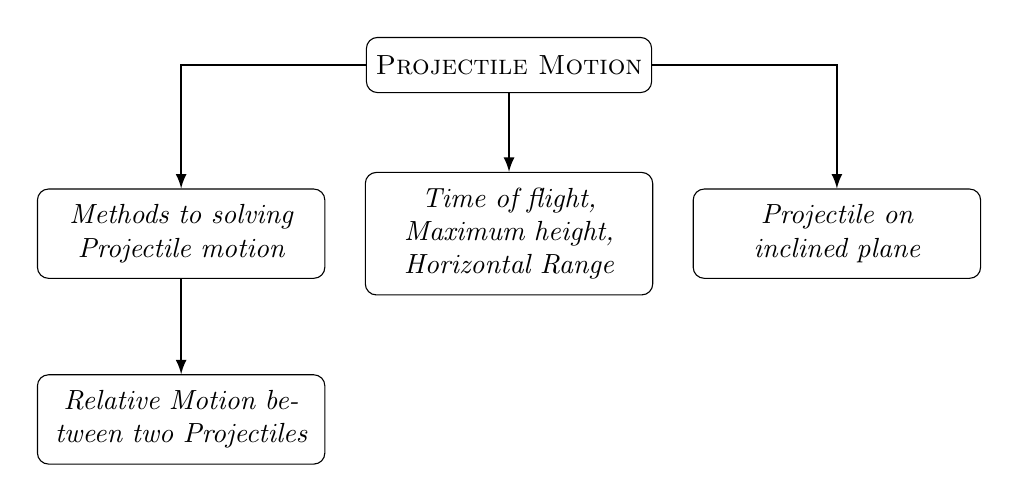
\begin{tikzpicture}[node distance=2cm]

\matrix [column sep=5mm,row sep=10mm]
{
&\node (root) [root] {Projectile Motion};\\
\node (child-left)[child] {Methods to solving Projectile motion}; &
\node (child-center)[child] {Time of flight, Maximum height, Horizontal Range}; &
\node (child-right)[child]{Projectile on inclined plane};\\
\node (child-left-b)[child] {Relative Motion between two Projectiles}; & &\\
};

\draw [arrow] (root) -| (child-left);
\draw [arrow] (root) -| (child-right);
\draw [arrow] (child-left) --(child-left-b);
\draw [arrow] (root)--(child-center);
\end{tikzpicture}
\end{center}

\begin{center}
    \textsc{Problems}
\end{center}
\begin{enumerate}
    \item Two particles are simultaneously projected in the same vertical plane from the same point with velocities $u$ and $v$ at angles $\alpha$ and $\beta$ with horizontal. Find the time that elapses when their velocities are parallel.	
	\begin{center}
	\begin{tikzpicture}
		\tzfn"curve"{-.25*(\x)^2+1*\x}[0:3]
		\pic[xshift=2cm] (0, 0) {frame=7cm};
		\tztangentat[->]{curve}{0.01}[0:1]{$u$}[ar]
		\tzvXpointat{curve}{0.01}(PG)
		\tzanglemark[->](1, 0)(0, 0)(PG){$\alpha$}(15pt)
		\begin{scope}[xshift=0cm]
			\tzfn"curve"{-.35*(\x)^2+1.5*\x}[0:3]
			\pic[xshift=2cm] (0, 0) {frame=7cm};
			\tztangentat[->]{curve}{0.01}[0:1]{$v$}[ar]
			\tzvXpointat{curve}{0.01}(PG)
			\tzanglemark[->](1, 0)(0, 0)(PG){$\beta$}(25pt)
		\end{scope}
	\end{tikzpicture}
	\end{center}
	\begin{tasks}(2)
		\task $t=\dfrac{uv\cos(\alpha-\beta)}{g(v\sin(\beta)-u\sin(\alpha))}$
		\task $t=\dfrac{uv\sin(\alpha-\beta)}{g(v\cos(\beta)-u\cos(\alpha))}$\ans
		\task $t=\dfrac{uv\sin(\alpha-\beta)}{g(v\sin(\beta)-u\sin(\alpha))}$
		\task $t=\dfrac{uv\cos(\alpha-\beta)}{g(v\cos(\beta)-u\cos(\alpha))}$
	\end{tasks}

    \item If the instantaneous velocity of a particle projected as shown in figure by $\Vec{v}=a\hat{i}+(b-ct)\hat{j}$. Where $a$, $b$ and $c$ are positive constants, the range on the horizontal plane will be
    \begin{center}
        \begin{tikzpicture}
        \pic[xshift=2.5cm, ] (0, 0) {frame=8cm};
        \tzparabola"curve"(0, 0)(2.5, 1.5)(5, 0);
        \tzvXpointat*{curve}{4.99}
        \tzvXpointat*{curve}{0.01}(PT)
        \tztangentat[->]{curve}{0.01}[0:0.8]{$\Vec{v}$}
        \tzanglemark[->](5, 0)(0, 0)(PT){$\theta$}[scale=0.8]
        \end{tikzpicture}
    \end{center}
    \begin{tasks}(2)
        \task $\dfrac{2ab}{c}$\ans
        \task $\dfrac{ab}{c}$
        \task $\dfrac{ac}{b}$
        \task $\dfrac{a}{2bc}$
    \end{tasks}

    \item A projectile is given an initial velocity of $(\hat{i} + 2\hat{j}) \mps$ where, $\hat{i}$ is along the ground and $\hat{j}$ is along the vertical. If $g = 10 \mpss$ , the equation of its trajectory is
	\begin{center}
	\begin{tikzpicture}
		\tzfn"curve"{-.25*(\x)^2+1*\x}[0:4]
		\pic[xshift=2cm] (0, 0) {frame=7cm};
		\tztangentat[->]{curve}{0.01}[0:1]{$\hat{i}+2\hat{j}$}[ar]
		\tzvXpointat{curve}{0.01}(PG)
		\tzanglemark[->](1, 0)(0, 0)(PG){$\theta$}(15pt)
	\end{tikzpicture}
	\end{center}
	\begin{tasks}(2)
		\task $y=x-5x^2$
		\task $y=2x-5x^2$\ans
		\task $4y=2x-5x^2$
		\task $4y=2x-25x^2$
	\end{tasks}
	
	\item A ball is projected upwards from the top of a tower with a velocity $50\mps$ making an angle $30^\circ$ with the horizontal. The height of tower is $70 \m$. After how many seconds from the instant of throwing, will the ball reach the ground. ($g = 10 \mpss$)	
	\begin{tasks}(2)
		\task $2\s$
		\task $5\s$
		\task $7\s$\ans
		\task $9\s$
	\end{tasks}
	
	
	
	\item A body is projected at time $t = 0$ from a certain point on a planet's surface with a certain velocity at a certain angle with the planet's surface (assumed horizontal). The horizontal and vertical displacements $x$ and $y$ (in metre) respectively vary with time $t$ in second as, $x = 10\sqrt{3}t$ and $y = 10t-t^2$. The maximum height attained by the body is
	\begin{tasks}(2)
		\task $75\m$
		\task $100\m$
		\task $50\m$
		\task $25\m$\ans
	\end{tasks}
	

    \item A body falling freely from a given height $H$ hits an inclined plane in its path at a height $h$. As a result of this impact, the velocity of the body becomes horizontal. For what value of $\dfrac{h}{H}$ will be body take maximum time to reach the ground?
        
        \begin{multicols}{2}
            \begin{tasks}(1)
                \task $\dfrac{h}{H} = \dfrac{1}{2}$\ans
                \task $\dfrac{h}{H} = \dfrac{1}{3}$
                \task $\dfrac{h}{H} = \dfrac{1}{4}$
                \task $\dfrac{h}{H} = \dfrac{1}{5}$
            \end{tasks}
            \begin{center}
                \begin{tikzpicture}
                    \pic at (-1.5,0) {frame=7cm};
                    \draw[dashed](0,0)--(0,3);
                    \tzfn{(-0.2*\x*\x)+3}[0:-3.9]
                    \pic[rotate=45] at (0,3) {frame=2cm};
                    \tzline+[->] (0,5)(0,-1)
                    \tzline+[->] (0,3)(-2,0)
                    \fill (0,5) circle(4pt);
                    \tzline+[|<->|]<1, 0>(0,0)(0,5){$H$}[midway, right]
                    \tzline+[|<->|]<0.5, 0>(0,0)(0,3){$h$}[midway, right]
                \end{tikzpicture}
            \end{center}
        \end{multicols}
        
	
	
	\item The maximum range of a bullet fired from a toy pistol, mounted on a car at rest is $R_0 = 40 \m$. What will be the acute angle of inclination of the pistol for maximum range when the car is moving in the direction of firing with uniform velocity $v = 20 \mps$, on a horizontal surface?($g=10\mpss$)
	\begin{tasks}(2)
		\task $30^\circ$
		\task $60^\circ$\ans
		\task $75^\circ$
		\task $45^\circ$
	\end{tasks}
	
	
	\item A particle is released from a certain height $H = 400 \m$. Due to the wind, the particle gathers the horizontal velocity component $v_x = \alpha y$ where $\alpha = 5 s^{-1}$ and $y$ is the vertical displacement of the particle from the point of release, then the horizontal drift of the particle when it strikes the ground is
	\begin{tasks}(2)
		\task $1.67\km$
		\task $3.67\km$
		\task $2.67\km$\ans
		\task $4.67\km$
	\end{tasks}
	
	
	
	\item A particle is projected along an inclined plane as shown in figure. What is the speed of the particle when it collides at point $A$ ? ($g = 10 \mpss$)
	\begin{center}
	\begin{tikzpicture}
		\tzfn"curve"{-.25*(\x)^2+1*\x}[0:3]
		\pic[xshift=2cm] (0, 0) {frame=7cm};
		\tztangentat[->]{curve}{0.01}[0:1]{$10\mps$}[ar]
		\tzvXpointat{curve}{0.01}(PG)
		\tzanglemark[->](1, 0)(0, 0)(PG){$60^\circ$}(15pt)
		\tzline(0, 0)(4, 1)
		\tzanglemark[->](1, 0)(0, 0)(4, 1){$30^\circ$}(25pt)
		\tznode(3, 0.75){$A$}[ar]
	\end{tikzpicture}
	\end{center}
	\begin{tasks}(2)
		\task $\dfrac{10}{\sqrt{3}}\mps$\ans
		\task $\dfrac{5}{\sqrt{3}}\mps$
		\task $\dfrac{15}{\sqrt{3}}\mps$
		\task $\dfrac{20}{\sqrt{3}}\mps$
	\end{tasks}
	
	
	\item A ball is projected from point $A$ with velocity $10 \mps$ perpendicular to the inclined plane as shown in figure. Range of the ball on the inclined plane is 
	\begin{center}
	\begin{tikzpicture}
	\def\t{4.25}
		\tzfn"curve"{-.5*(\x)^2+2.5*\x+0.5}[-0.05:\t + 0.01]
		\pic[xshift=1.5cm] (0, 0) {frame=7cm};
		\tztangentat[->]{curve}{\t}[\t:2.8]{$10\mps$}[a]
		\tzvXpointat*{curve}{\t}(PG){$A$}[r]
		\tzvXpointat{curve}{\t - 0.01}(PT)
		\tzline(-1, 0)(PG)
		\tzanglemark[->](1, 0)(-1, 0)(PG){$30^\circ$}(25pt)
		\tzrightanglemark(PT)(PG)(-1, 0){$90^\circ$}
	\end{tikzpicture}
    \vspace*{-10mm}
	\end{center}
	\begin{tasks}(2)
		\task $\dfrac{40}{3}\m$\ans
		\task $\dfrac{20}{3}\m$
		\task $\dfrac{12}{3}\m$
		\task $\dfrac{60}{3}\m$
	\end{tasks}
	
	\item In the figure shown, the two projectiles are fired simultaneously. The minimum distance between them during their flight is
	\begin{center}
	\begin{tikzpicture}
		\pic[xshift=2.5cm] (0, 0) {frame=8cm};
		\tzcoors(0, 0)(O)(1, 1.8)(A)(5, 0)(O')(3.5, 1.5)(A');
		\tzline[->](O)(A){$20\sqrt{3}\mps$}[a]
		\tzline[->](O')(A'){$20\mps$}[a]
		\tzanglemark[->](O')(O)(A){$60^\circ$}(15pt)
		\tzanglemark[->](A')(O')(O){$30^\circ$}(15pt)
		\tzline[|<->|]<0, -0.5>(O)(O'){$20\sqrt{3}\m$}[b, midway]
	\end{tikzpicture}
	\end{center}
	\begin{tasks}(2)
		\task $20\m$
		\task $10\sqrt{3}$\ans
		\task $10\m$
		\task None of these
	\end{tasks}
	

    \item The trajectories of the motion of three particles are shown in the figure. Match the entries of Column I with the entries of Column II. Neglect air resistance.
    \begin{center}
        \begin{tikzpicture}
            \tzaxes(0, 0)(7, 4){$x$}{$y$}
            \tzline[dashed](0, 3)(3.5, 3)
            \tzparabola[-->--=0.3, -->--=0.7](0, 0)(1.5, 3)(3, 0){$A$}[al=5mm]
            \tzparabola[-->--=0.3, -->--=0.7](0, 0)(2, 3)(4, 0){$B$}[al=5mm]
            \tzparabola[-->--=0.3, -->--=0.7](0, 0)(2.5, 3)(5, 0){$C$}[al=5mm]
        \end{tikzpicture}
    \end{center}
    \begin{center}
        \renewcommand{\arraystretch}{1.5}
        \begin{tabular}{p{8cm}|p{4cm}}
        \hline
        Column I & Column II \\
        \hline
        (a) Time of flight is least for & (p) $A$\\
        (b) Vertical component of velocity is greatest for & (q) $B$\\
        (c) Horizontal component of velocity is greatest for & (r) $C$\\
        (d) Launch speed is least for & (s) same for all\\
        \hline
        \end{tabular}
    \end{center}
    \begin{tasks}(2)
        \task $(a) \rightarrow(s), (b) \rightarrow(s), (c) \rightarrow(r), (d) \rightarrow(p)$\ans
        \task $(a) \rightarrow(r), (b) \rightarrow(q), (c) \rightarrow(p), (d) \rightarrow(s)$
        \task $(a) \rightarrow(p), (b) \rightarrow(s), (c) \rightarrow(r), (d) \rightarrow(q)$
        \task $(a) \rightarrow(p), (b) \rightarrow(q), (c) \rightarrow(r), (d) \rightarrow(s)$
    \end{tasks}

    \begin{center}
        \textsc{Comprehension Based Questions}
    \end{center}
    Two inclined planes OA and OB intersect in a horizontal plane having their inclinations $\alpha$ and $\beta$ with the horizontal as shown in A figure. A particle is projected from point P with velocity $u$ along a direction perpendicular to plane OA. The particle strikes plane OB perpendicularly at Q.
    \begin{center}
        \begin{tikzpicture}
            \tzcoor(0, 0)(O){$O$}[b]
            \pic at (O) {frame=9cm};
            \tzline+(O)(150:4){$A$}[l]
            \tzline+(O)(30:4){$B$}[r]
            \tzline+[->]($(O)+(150:3.5)$)(60:1){$u$}[a]
            \tzline+[<-]($(O)+(30:3.5)$)(120:1)
            \tzanglemark(2, 0)(O)(30:3){$\beta$}(15pt)
            \tzanglemark(150:3)(O)(-2, 0){$\alpha$}(15pt)
            \tzline[|<->|]<30:0.15>(O)(150:3.5){$a$}[ma]
        \end{tikzpicture}
    \end{center}
    \item If $\alpha=30^\circ$, $\beta=30^\circ$, the time of flight from $P$ to $Q$ is
    \begin{tasks}(2)
        \task $\dfrac{2u}{g}$
        \task $\dfrac{\sqrt{3}u}{g}$\ans
        \task $\dfrac{u}{2g}$
        \task $\dfrac{u}{3g}$
    \end{tasks}

    \item If $\alpha=30^\circ$, $\beta=30^\circ$, and $a=4.9\m$, the initial velocity of projection is
    \begin{tasks}(2)
        \task $9.8\mps$\ans
        \task $4.9\mps$
        \task $4.9\sqrt{2}\mps$
        \task $19.6\mps$
    \end{tasks}
	
\end{enumerate}


\pagebreak

\begin{center}
\texttt{Answer Key}
\begin{multicols}{5}
\begin{enumerate}
\item (b)
\item (a)
\item (b)
\item (c)
\item (d)
\item (a)
\item (b)
\item (c)
\item (a)
\item (a)
\item (b)
\item (a)
\item (b)
\item (a)
\end{enumerate}
\end{multicols}
\end{center}






\end{document}